% vim:set textwidth=100:
% vim:set fo+=t:


\documentclass[10pt]{article}

\usepackage{amsmath}
\usepackage[nofiglist,notablist]{endfloat}
\usepackage[usenames,dvipsnames]{color}
\usepackage{color}
\usepackage{authblk}
\usepackage{graphicx}
\usepackage{palatino}
\usepackage[activate={true,nocompatibility},final]{microtype}
\usepackage[super,sort&compress]{natbib}
\pagenumbering{arabic}
\parskip = 0.08in \parindent = 0.0in 

% Custom macros for author comments
\newcommand{\Alberto}[1]{\color{ForestGreen}Alberto: #1 \normalcolor }
\newcommand{\Justin}[1]{\color{blue}Justin: #1 \normalcolor}
\newcommand{\Arijit}[1]{\color{yellow}Arijit: #1 \normalcolor}
\newcommand{\Ken}[1]{\color{red}Ken: #1 \normalcolor}

\author{Alberto~Perez$^2$}
\author{Ivet~Bahar$^1$}
\author{Ken~A.~Dill$^2$}
\author{Justin~L.~MacCallum$^2$}
\affil{$^1$Department of Computational and Systems Biology, and Clinical \& Translational Science
    Institute, School of Medicine, University of Pittsburgh, 3064 BST3, 3501 Fifth Ave, Pittsburgh,
    PA 15213}
\affil{$^2$Laufer Center for Physical and Quantitative Biology\\
    Stony Brook University\\
    Stony Brook, NY 11794-5252}

\title{Title}

\begin{document}

\maketitle
\begin{abstract}
%How to cite something in paper.bib
    Abstract \citep{CASP9}

\end{abstract}


\section{Introduction}


%this is how you put a figure in document
\begin{figure} \centering 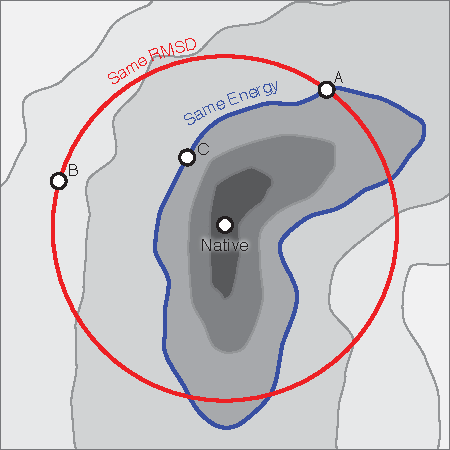
\includegraphics[width=3in]{rmsd_energy_schematic2.pdf}

    \caption{Schematic}

    \label{fig:conf_schematic} 
\end{figure}

\section{Methods}

\subsection{ENM}

%this is how you put a table
\begin{table} 
    \centering
    \caption{Structures used for large motions}
    \label{tbl:targets}
    \begin{tabular}{l l l}
    \hline
    Target                           & PDB1 & PDB2 \\
    \hline
	Scallop myosin                   & 1kk7 & 1kk8 \\
	Acyl Carrier Protein             & 1acp & 2fae \\
	Aspartate Aminotransferase       & 1ama & 8aat \\
	Bcl-xl                           & 1bxl & 1ysn \\
	Calcium Sensor                   & 1k9k & 1k9p \\
	Calmodulin                       & 1cll & 1ctr \\
	Cyclin Dependent Kinase Inhibitor & 1dc2 & 2a5e \\
	Cystatin                         & 1a67 & 1cew \\
	%CytCOxidase                     & 1oco & 2occ \\
	Hydrolase                        & 1qz3 & 1u4n \\
	LacRepressor                     & 1lcc & 1lqc \\
	LambdaCro                        & 5cro & 6cro \\
	Lupin Hydrolase                  & 1f3y & 1jkn \\
	Maltose Binding Protein          & 1omp & 3mbp \\
	Pin1                             & 1f8a & 1pin \\
	%Thrombin                        & 1avg & 1ett \\
        \hline
    \end{tabular}
\end{table}

%This tells latex to reference the figure or table
See figure \ref{fig:conf_schematic}.

See table \ref{tbl:targets}.

\bibliographystyle{achemso} 
\bibliography{paper}

\end{document}
